\chapter{CH$_{3}$NH$_{2}$ survey in low mass star-forming regions
\label{chap:appendixA}}

CH$_{3}$NH$_{2}$ survey in low mass star-forming regions is also significant, 
as the low mass star- formation region is considered to be directly related to the origin of the comets. 
We surveyed not only in Orion-KL but also in the following two low mass star-forming regions, 
but CH$_{3}$NH$_{2}$ was not detected.  
Therefore, we evaluated the upper limit to its column densities as a function of rotational temperature 
by using the intensity of 3 noise level. 
We used lines whose $S\mu^2$ value is large  in relatively line free regions.
We report the results of the analysis briefly.

\section{IRAS 16293}
IRAS 16293 is a binary system of two stars, of which source B has narrower line width 
($\sim$ 1.0 km s$^{-1}$) and is suitable for line survey \citep{Persson+2018}. 
The CH$_{3}$NH$_{2}$ survey in this region has been done \citep{Ligterink+2018}, 
but CH$_{3}$NH$_{2}$ was not detected.
In this paper, they used ALMA  band 7 data and analyzed the spectrum extracted from an offset position toward source B.
Therefore, we performed additional analysis in other band without applying spatial bias. 
The line survey procedure is the same up to no.2 in Section 2.2.2.

\subsection{Observation data}
ALMA Band 6 archive data of PILS survey was used (\#2012.1.00712.S, \citet{Jorgensen+2016}).
These data cube were already calibrated by \citet{Oya+2016}.  
The backend correlator was tuned to a resolution of 122 kHz, which corresponds to a
velocity resolution of 0.15 km s$^{-1}$ at 240 GHz.
Details of each data are summarized in Table \ref{tab:Obs_IRAS16293}.

\renewcommand{\arraystretch}{1.5}
\begin{table}[htb]
\begin{center}
  \caption{Summary of Observations for IRAS 16293}
  \label{tab:Obs_IRAS16293}
{\scriptsize
  \begin{tabular}{lllllll} \hline \hline
 & Window & Frequency range [GHz] & Date & FWHM & PA \\ \hline
 B6-1 & 0 & 239.40-239.86 & 2014-Jun.-14 & 0.48''$\times$0.43'' & 15\\
 & 1 & 240.15-240.51 & & & \\
 & 2 & 224.75-225.21 & & & \\
 & 3 & 221.76-222.22 & & & \\ \hline
 B6-2 & 0 & 247.32-247.79 & 2014-May.-22 & 0.62''$\times$0.48'' & 77\\
 & 1 & 250.28-250.75 & & & \\
 & 2 & 231.03-231.51 & & & \\
 & 3 & 232.18-232.65 & & & \\ \hline
  \end{tabular}
  }
\end{center}
\end{table}

\subsection{Results}
There were 4 CH$_{3}$NH$_{2}$ emission lines that were predicted not to be contaminated 
by other molecular emission lines within the observation frequency coverage, 
but in any case, radiation exceeding 3 $\sigma$ noise level were not be confirmed.
Figure \ref{IRAS16293_mom0} is an example of integrated intensity map.
Since FWHM line width of IRAS 16293 B is $\Delta V_{1/2} \sim$ 1.0 km s$^{-1}$ and 1$\sigma=$ 3.8 mJy, 
signals less than 11.4~mJy~beam$^{-1}$~km~s$^{-1}$ are not regarded as significant.

\begin{figure}[htp]
  \centering
  \includegraphics[width=0.65\textwidth]{LMSFR/IRAS16293_mom0.eps}
  \caption{Integrated intensity map around 247.362 GHz. The white contours represent the 1.3 mm continuum map, where the contour levels are 10 \%, 30 \%, 50 \%, 70 \%, 90 \% of the peak intensity of 0.65 Jy/beam.}
  \label{IRAS16293_mom0}
\end{figure}

The column density can be obtained by transforming Equation \ref{eq:RD} as follows.
\begin{align}
N_{\mathrm{MA}} = U_{\mathrm{rot}} \times \dfrac{3\,k_{\mathrm{B}}\,T_{\mathrm{B}} \,\Delta V_{1/2}}{8\, \pi^3\, \nu\, S\, \mu_0^2} \times 10^{E_{\mathrm{u}}/k_{\mathrm{B}}\,T_{\mathrm{rot}}} \times e
\label{eq:N_MA}
\end{align}

The upper limit column densities of CH$_{3}$NH$_{2}$ have been
determined for rotational temperatures between 70 and 130 K.
These are plotted in Figure \ref{IRAS16293_MA}.
The upper limit column densities of CH$_{3}$NH$_{2}$ are determined on the
$7_{2}E_{1-1} \rightarrow 7_{1}E_{1-1}$ transition at 247.362 GHz ($S\mu^2 = 33.68$ D$^2$) for a 3$\sigma$ line intensity of 3.8~mJy~beam$^{-1}$.

\begin{figure}[htp]
  \centering
  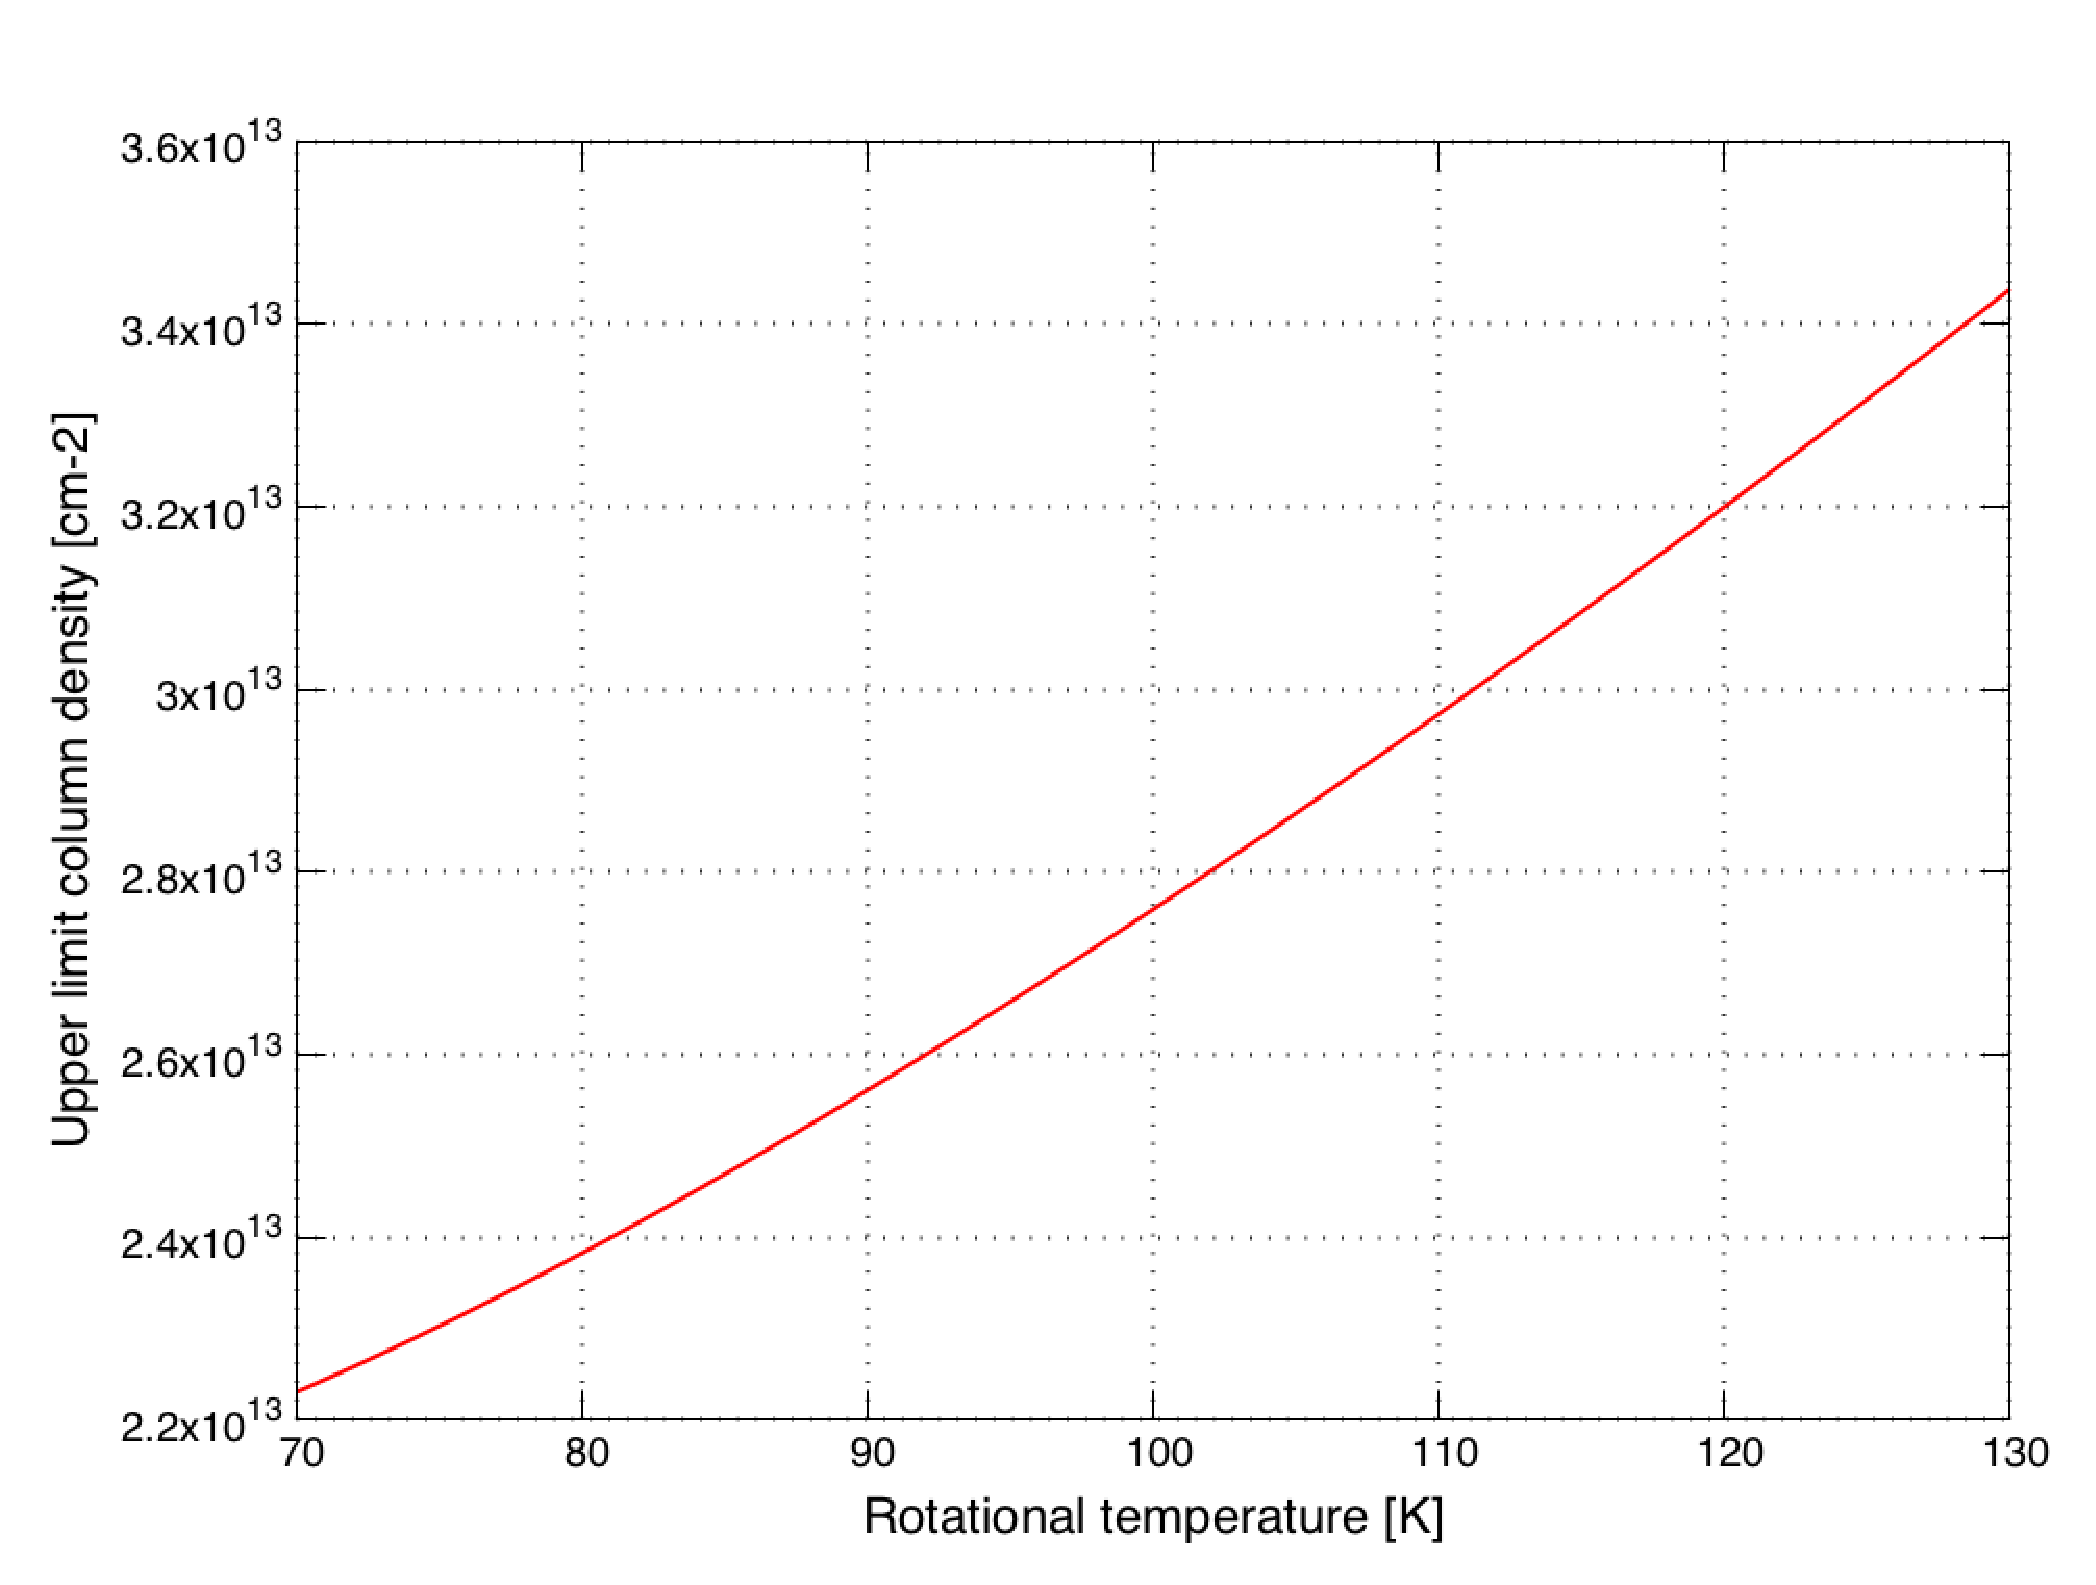
\includegraphics[width=0.7\textwidth]{LMSFR/IRAS16293.eps}
  \caption{Upper limit column density for the strongest CH$_{3}$NH$_{2}$ transition
  ($7_{2}E_{1-1} \rightarrow 7_{1}E_{1-1}$) as function of T$_{\textrm{rot}}$. A 3$\sigma$ value of 
  11.4 mJy beam$^{-1}$ is used.}
  \label{IRAS16293_MA}
\end{figure}

The order of the obtained value of CH$_{3}$NH$_{2}$ was about 13.
Compared to the column density of detected N-bearing COMs 
\citep[e.g., 4.4$^{+3.0}_{-1.9}$ $\times$ 10$^{14}$ cm$^{-2}$ for NH$_2$CHO,][]{Kahane+2013}, 
the upper limit of CH$_{3}$NH$_{2}$ seems to be consistent.


\section{L483}
CH$_{3}$NH$_{2}$ survey in L483 has not been reported so far.
Therefore we attempted exploration of CH$_{3}$NH$_{2}$ for the first time using ALMA Band 6 archive data (\#2016.1.01325.S. PI: Yoko Oya).

\subsection{Observation data}
ALMA data cube were already calibrated and reduced by Oya et al. 
Details of each data are summarized in Table \ref{tab:Obs_L483}

\renewcommand{\arraystretch}{1.5}
\begin{table}[htb]
\begin{center}
  \caption{Summary of Observations for L483}
  \label{tab:Obs_L483}
{\scriptsize
  \begin{tabular}{llc} \hline \hline
  Window & Frequency range [GHz] & Channel width [KHz]  \\ \hline
0&217.054675-217.113267&122.07 \\
1&218.188881-218.247473&122.07\\
2&218.4246824-218.483274&122.07\\
3&218.7137034-218.772295&122.07\\
4&219.5166704-219.575262&122.07\\
5&219.7756644-219.834256&122.07\\
6&219.9161004-219.974692&122.07\\
7&220.7136484-220.772240&122.07\\
8&236.479210-236.5378016&122.07\\
9&235.124431-235.1830226&122.07\\
10&235.944439-236.0030306&122.07\\
11&236.701431-236.7600226&122.07\\
12&232.748687-232.9830534&488.28\\
13&232.466563-232.7009295&488.28\\
14&244.5532143-244.611806&122.07\\
15&243.8820343-243.940626&122.07\\
16&244.2362093-244.294801&122.07\\
17&244.9017733-244.960365&122.07\\
18&247.1782195-247.412586&488.28\\
19&245.5792095-245.813576&488.28\\
20&262.359554-262.4181457&122.07\\
21&262.181917-262.2405087&122.07\\
22&263.708901-263.8260843&122.07\\
23&261.795953-261.8545447&122.07\\
24&260.496957-260.5555487&122.07\\
25&262.057967-262.1165587&122.07\\
26&261.282971-261.3415627&122.07\\ \hline
  \end{tabular}
  }
\end{center}
\end{table}

\subsection{Results}
There were 12 CH$_{3}$NH$_{2}$ emission lines that were predicted not to be contaminated 
by other molecular emission lines within the observation frequency coverage, 
but in any case, radiation exceeding 3$\sigma$ noise level were not be confirmed.
Figure \ref{L483_mom0} is an example of integrated intensity map.
The rms noise level of this data was 7.5 mJy.
Assuming FWHM line width of L483 is $\Delta V_{1/2} \sim$ 6.0 km s$^{-1}$ \citep{Oya+2017}, 
signals less than 135~mJy~beam$^{-1}$~km~s$^{-1}$ are not regarded as significant.

\begin{figure}[htp]
  \centering
  \includegraphics[width=0.7\textwidth]{LMSFR/L483_mom0.eps}
  \caption{Integrated intensity map around 217.079 GHz. The white contours represent the 1.3 mm continuum map, where the contour levels are 10 \%, 30 \%, 50 \%, 70 \%, 90 \% of the peak intensity of 11 mJy/beam.}
  \label{L483_mom0}
\end{figure}

Similar to IRAS 16293 B, the upper limit column densities of CH$_{3}$NH$_{2}$ have been
determined for rotational temperatures between 70 and 130 K.
The upper limit column densities of CH$_{3}$NH$_{2}$ are determined on the
$11_{2}A_{1} \rightarrow 11_{1}A_{2}$ transition at 217.079 GHz ($S\mu^2 = 39.11$ D$^2$) for a 3$\sigma$ line intensity of 22.5 mJy beam$^{-1}$.
These are plotted in Figure~\ref{L483_MA}.

\begin{figure}[htp]
  \centering
  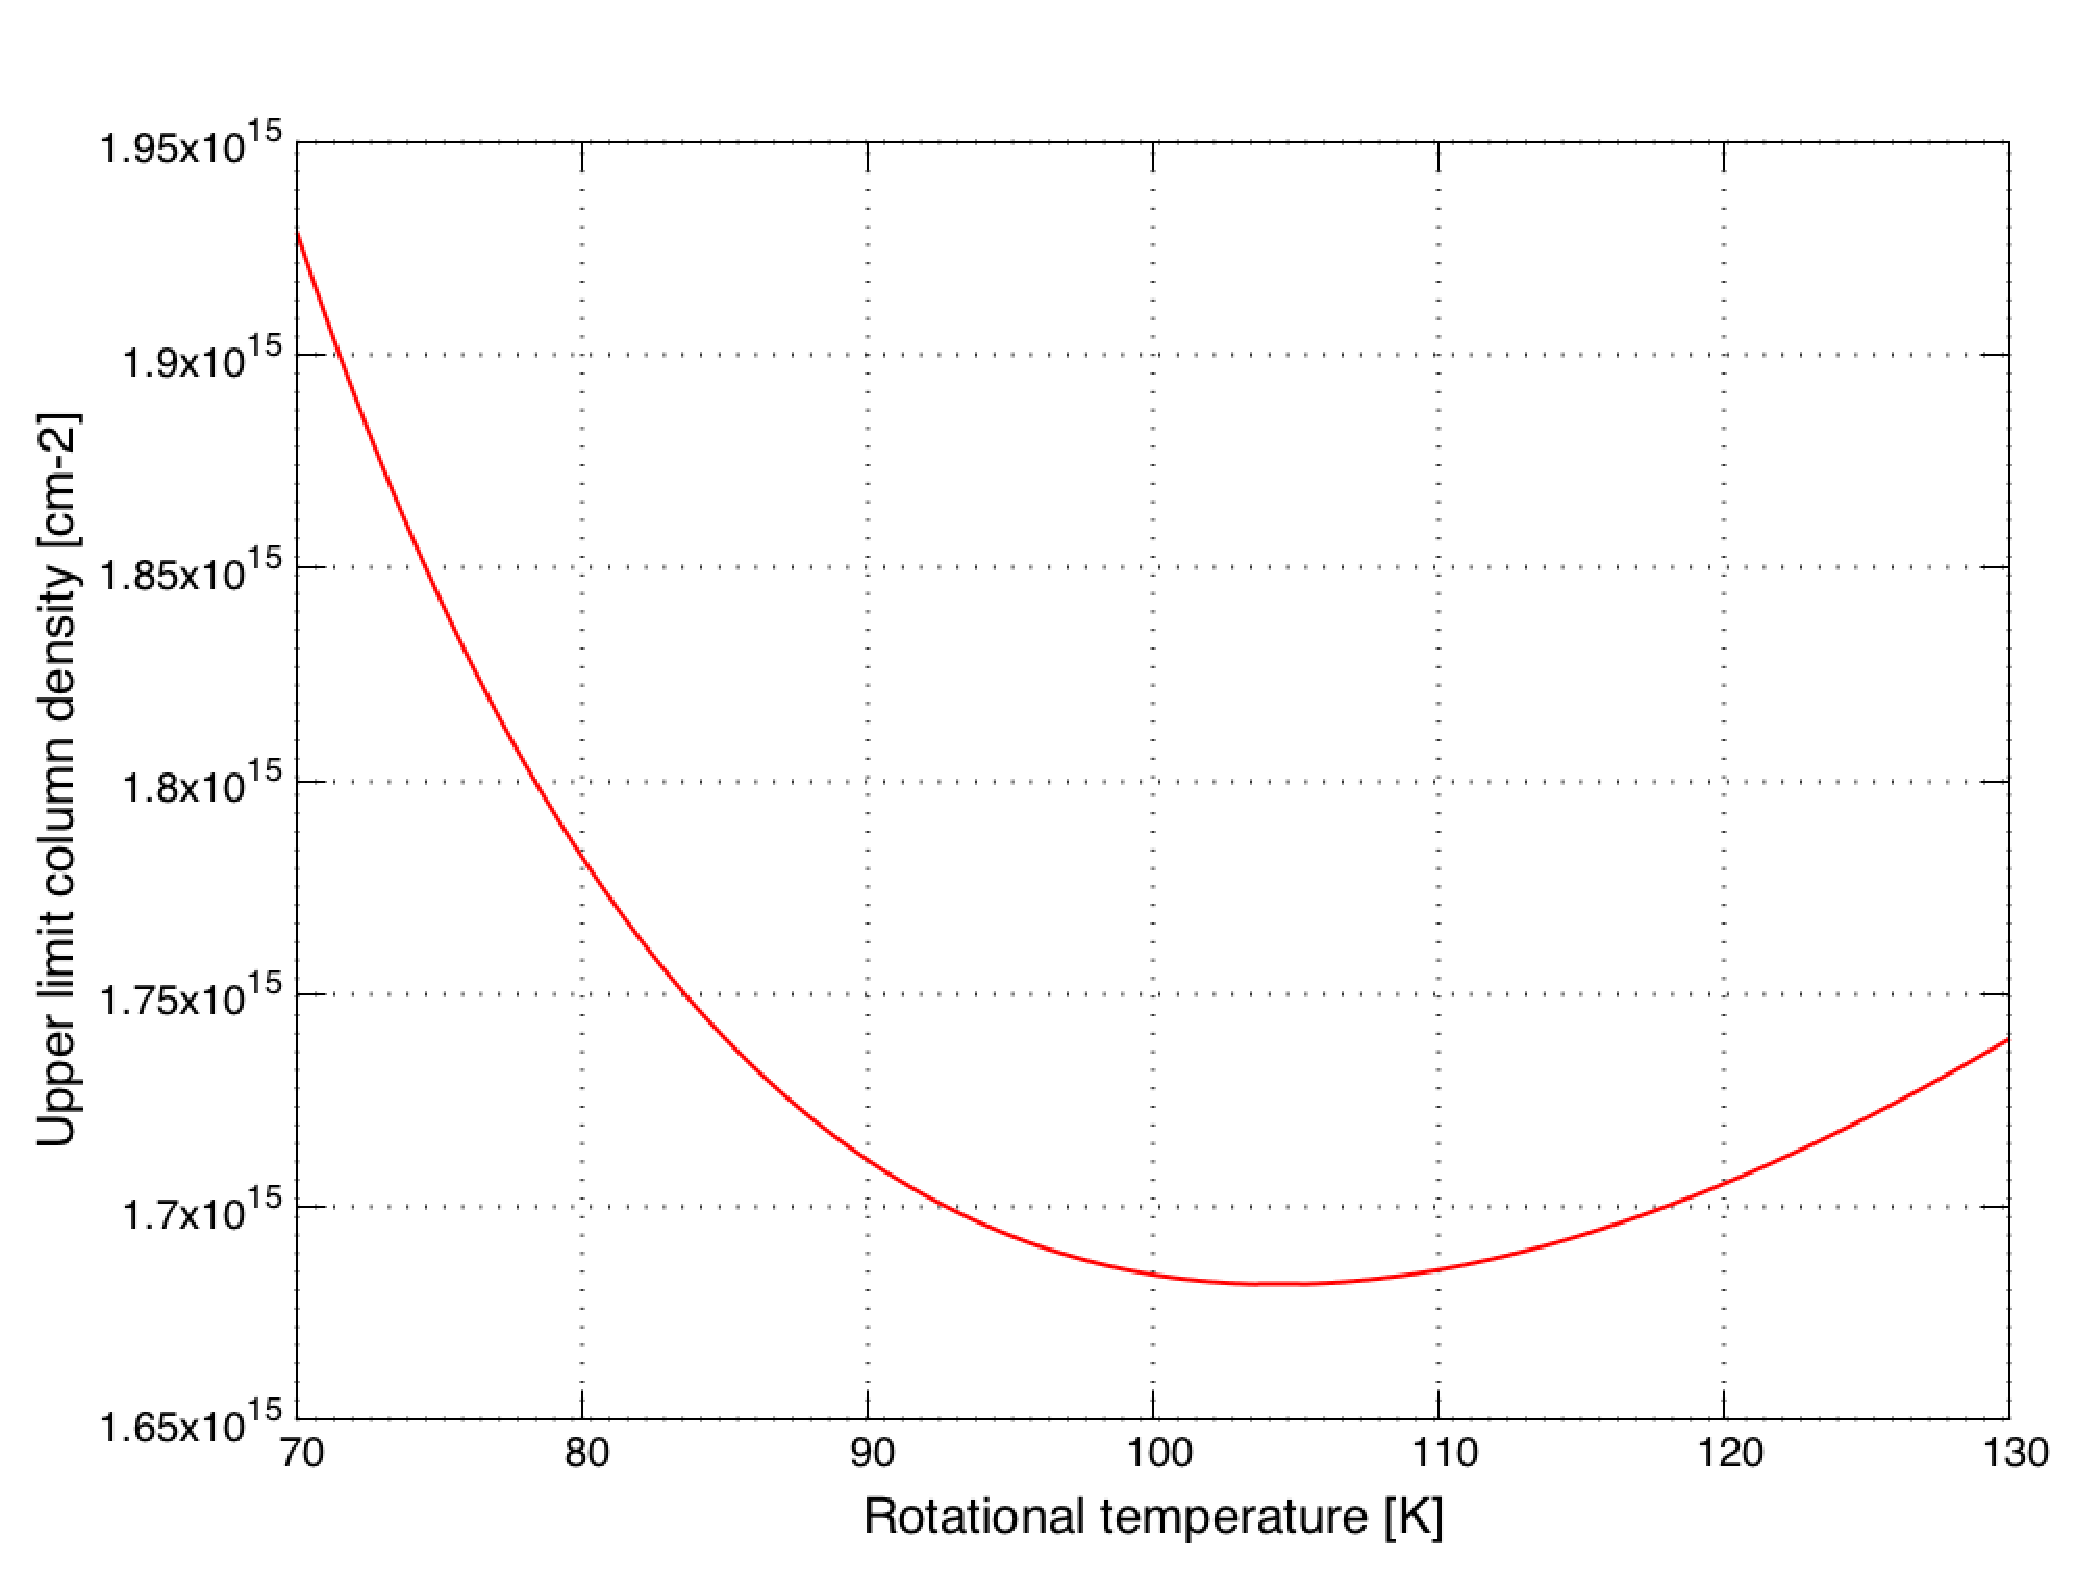
\includegraphics[width=0.7\textwidth]{LMSFR/L483.eps}
  \caption{Upper limit column density for the strongest CH$_{3}$NH$_{2}$ transition
  ($11_{2}A_{1} \rightarrow 11_{2}A_{2}$) as function of T$_{\textrm{rot}}$. A 3$\sigma$ value of 
  22.5 mJy beam$^{-1}$ is used.}
  \label{L483_MA}
\end{figure}

The order of the obtained value of CH$_{3}$NH$_{2}$ was about 15.
Compared to the column density of detected N-bearing COMs 
\citep[e.g., 1.2$\sim$1.9 $\times$ 10$^{14}$ cm$^{-2}$ for NH$_2$CHO,][]{Oya+2017}, 
the upper limit of CH$_{3}$NH$_{2}$ seems to be overestimated.
This overestimation seems to be derived from inappropriate line width selection.
According to \citet{Oya+2017}, it has been found that molecules trace different region, so that the line width is different. 
$\Delta V_{1/2} \sim$ 6.0 km s$^{-1}$ was derived from the simple molecules.
Since the line width of N-bearing species is narrow, it is estimated that the actual upper limit would be smaller.